
\appendix
\chapter{Konceptuální datový model}
\begin{figure}[htbp!]
	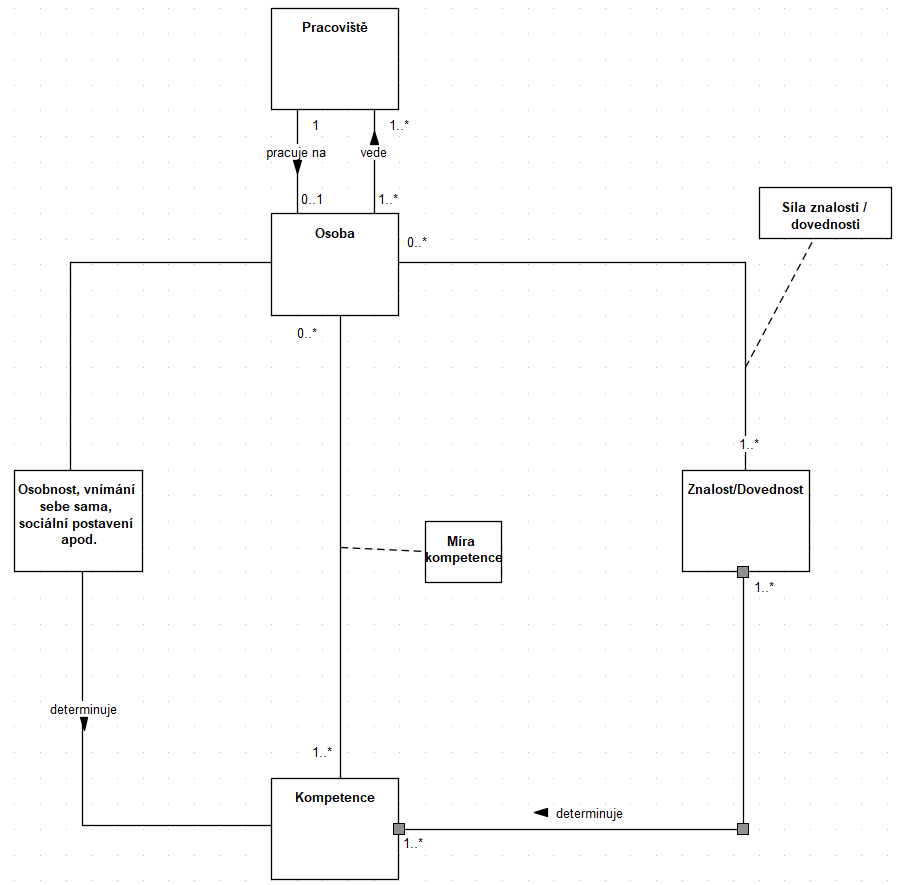
\includegraphics[width=\linewidth]{img/data_diagram.png}
	\caption{Diagram konceptuálního modelu (zdroj autor)}
	\label{fig:conceptual_appendix}
\end{figure}

% \chapter{Příklad ontologie}
% \begin{sidewaysfigure}[htbp!]
% 	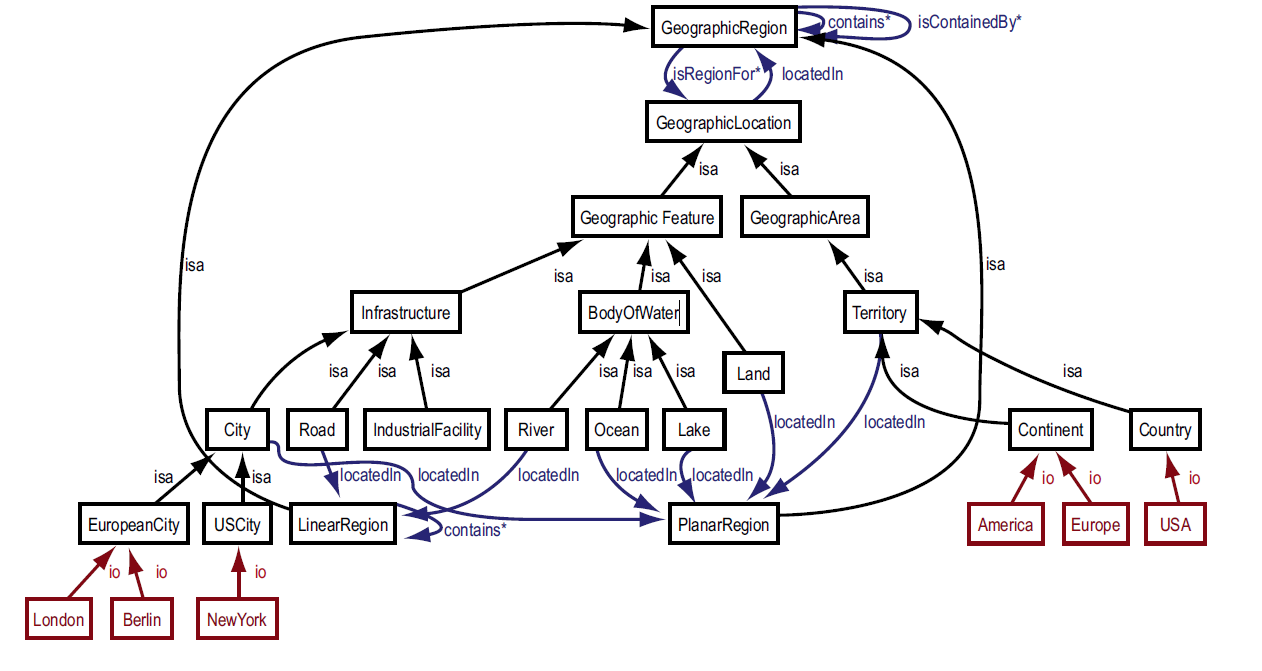
\includegraphics[width=0.75\linewidth]{img/ontology.png}
% 	\caption{Příklad geografické ontologie (zdroj \cite{Stephan2007})}
% 	\label{fig:ontology_example}
% \end{sidewaysfigure}

\chapter{SKOS vizualizace}
\begin{sidewaysfigure}[htbp!]
	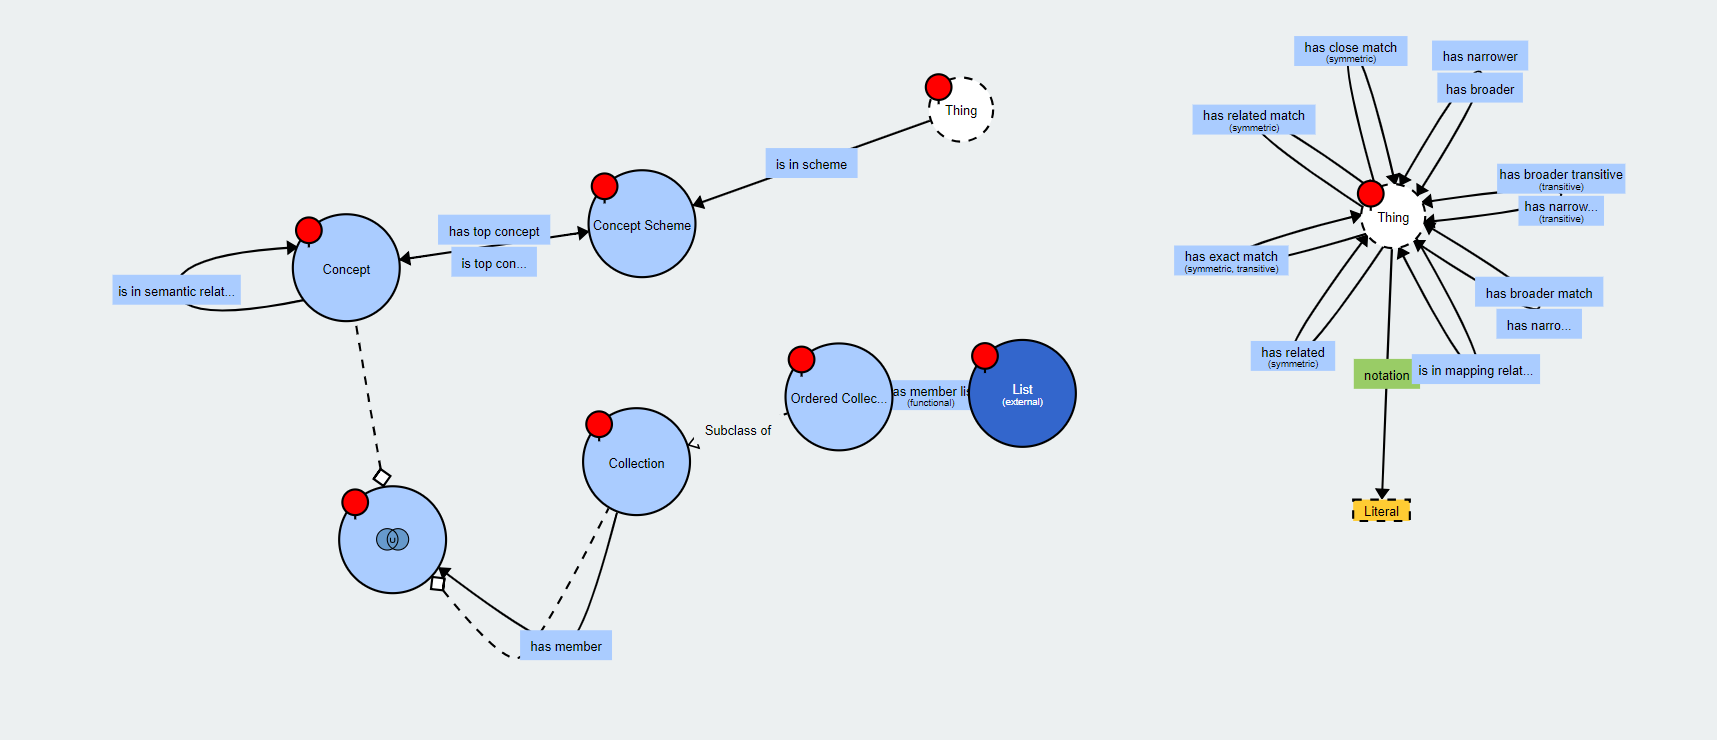
\includegraphics[width=0.9\linewidth]{img/SKOS-ontology.png}
	\caption{Ontologie SKOS (zdroj: \url{https://www.w3.org/2009/08/skos-reference/skos.rdf} použitý nástroj: \url{http://www.visualdataweb.de/webvow})}
	\label{fig:SKOS-ontology}
\end{sidewaysfigure}

\chapter{Diagram komponent}
\begin{sidewaysfigure}[htbp!]
	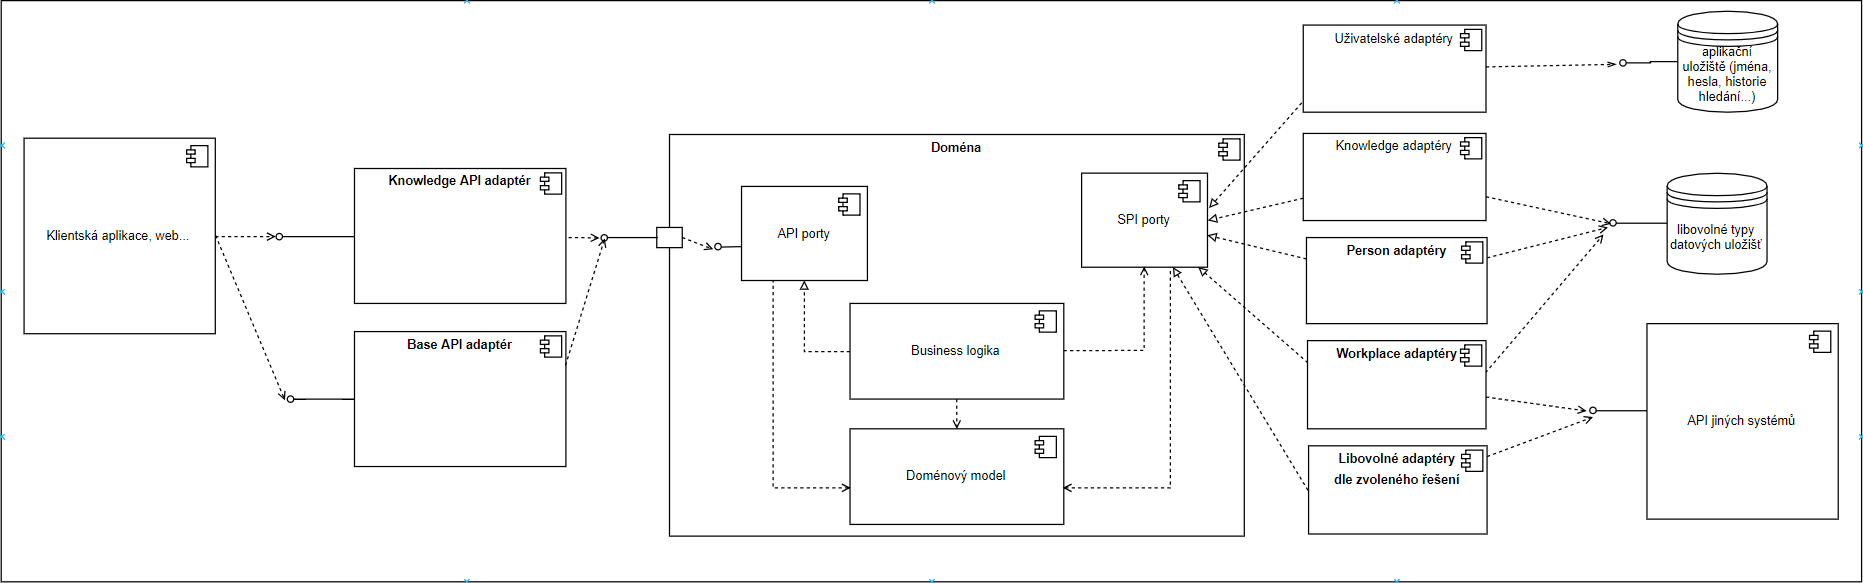
\includegraphics[width=\linewidth]{img/component.png}
	\caption{Diagram komponent (zdroj autor)}
	\label{fig:component-model}
\end{sidewaysfigure}

\chapter{Sekvenční diagram}  \label{appendix:sequence}
\begin{sidewaysfigure}[htbp!]
	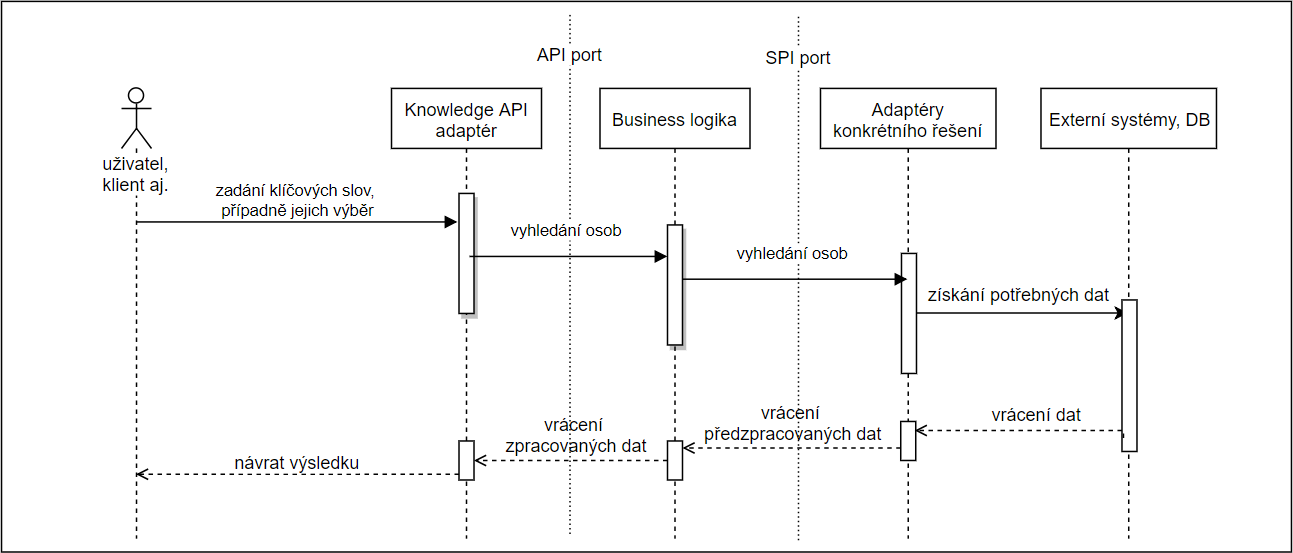
\includegraphics[width=\linewidth]{img/sequence-synchronous.png}
	\caption{Synchronní verze sekvenčního diagramu (zdroj autor)}
	\label{fig:sequence-synchronous}
\end{sidewaysfigure}

\begin{sidewaysfigure}[htbp!]
	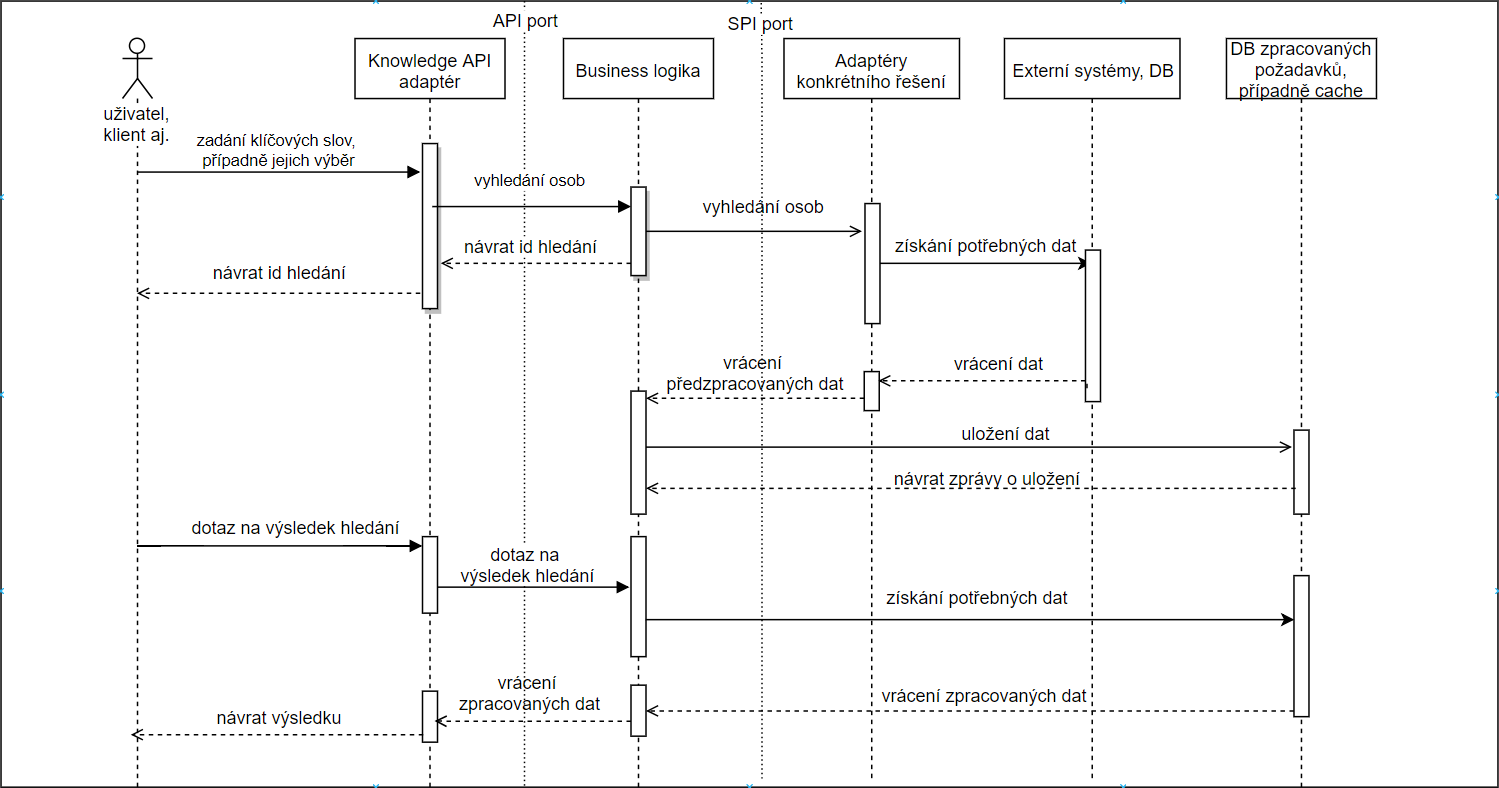
\includegraphics[width=\linewidth]{img/sequence-asynchronous.png}
	\caption{Asynchronní verze sekvenčního diagramu (zdroj autor)}
	\label{fig:sequence-asynchronous}
\end{sidewaysfigure}

\chapter{Doménový model}
\begin{figure}[htbp!]
	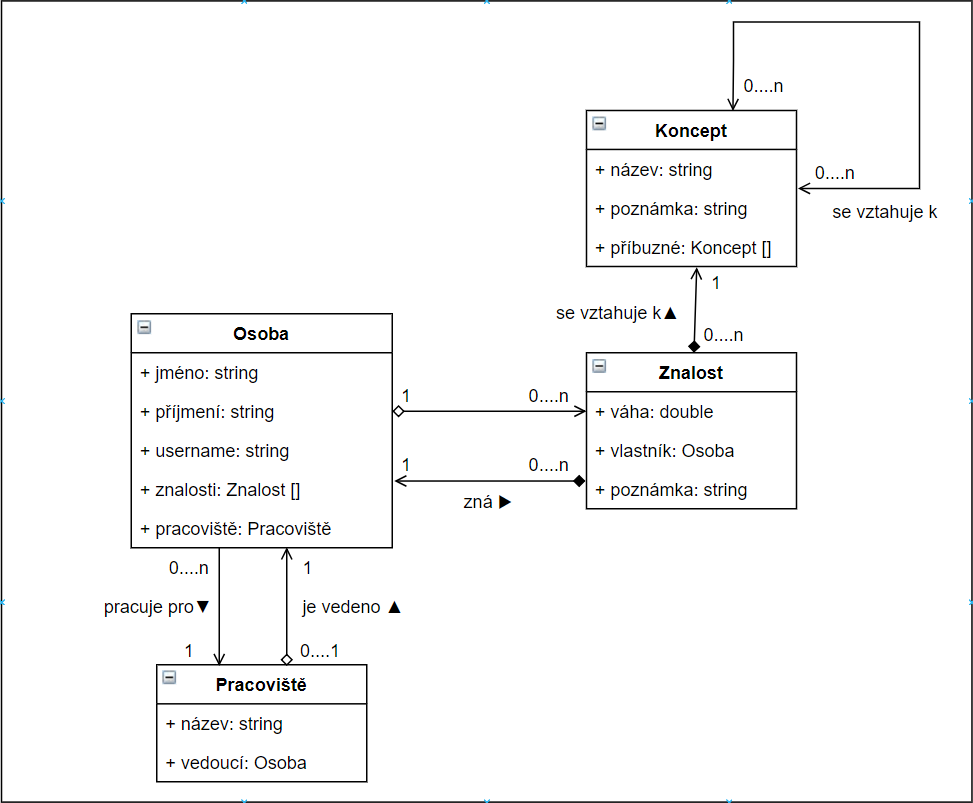
\includegraphics[width=\linewidth]{img/domain.png}
	\caption{Doménový model (zdroj autor)}
	\label{fig:domain-model}
\end{figure}

\chapter{Diagram komponent pro naše řešení FEL ČVUT}
\begin{sidewaysfigure}[htbp!]
	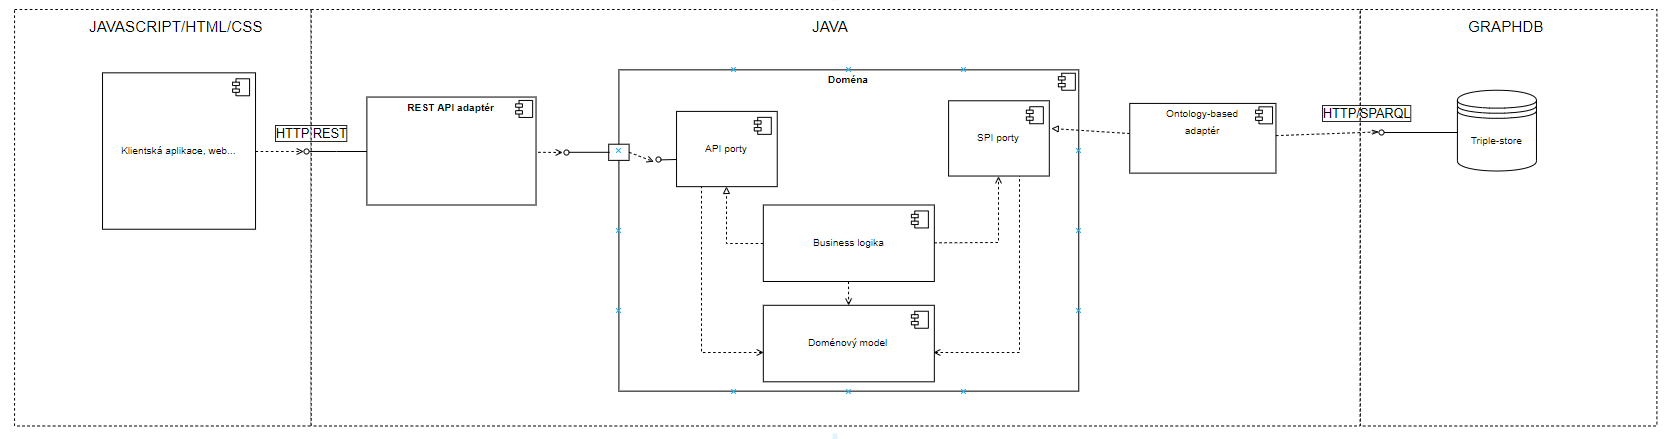
\includegraphics[width=\linewidth]{img/component-model-graphDB.png}
	\caption{Diagram komponent pro naše řešení (zdroj autor)}
	\label{fig:component-graphDB}
\end{sidewaysfigure}

\chapter{Ontologické schéma}
\begin{sidewaysfigure}[htbp!]
	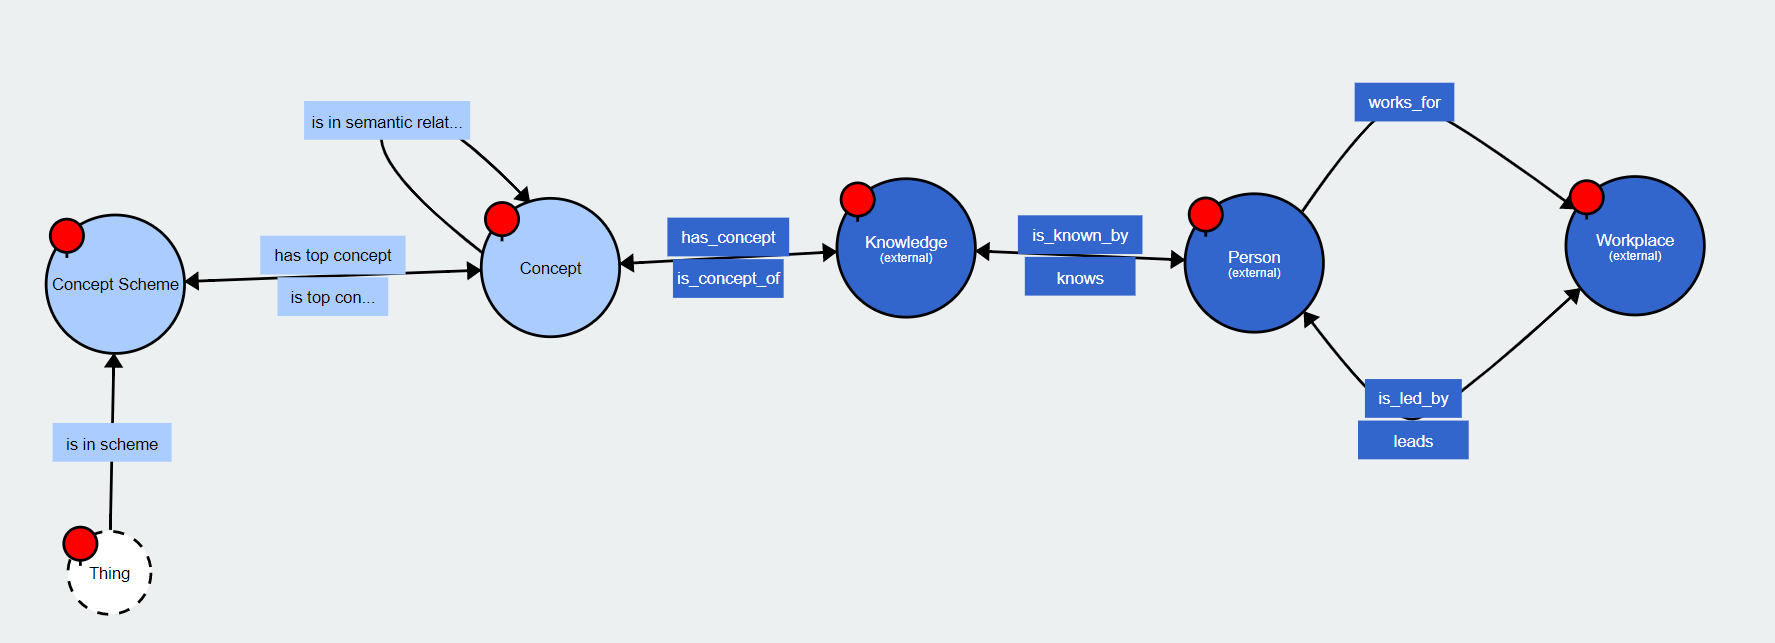
\includegraphics[width=\linewidth]{img/ontology-scheme.png}
	\caption{Použité ontologické schéma (zdroj autor, použitý nástroj \url{http://www.visualdataweb.de/webvowl/})}
	\label{fig:ontology-scheme}
\end{sidewaysfigure}

\chapter{SPARQL dotaz - vyhledávání osob dle kompetencí} \label{app:sparql-query}
\begin{lstlisting}[language=SPARQL, caption= SPARQL dotaz pro vyhledávání osob dle jejich kompetencí, captionpos=b]
    select ?person ?name ?surname ?username ?weight ?sub
    ?sub2 ?sub3 ?sub4 where {
         {
                ?person ?knows              ?k;
                        ?hasName            ?name;
                        ?hasUsername        ?username;
                        ?hasSurname         ?surname .
                ?k      ?hasWeight          ?weight;
                        ?hasConcept         ?concept .
        }
        UNION
        {
                ?person ?knows              ?k;
                        ?hasName            ?name;
                        ?hasUsername        ?username;
                        ?hasSurname         ?surname .
                ?k      ?hasWeight          ?weight;
                        ?hasConcept         ?sub1 .
                ?sub1   ?semanticRelation   ?concept .
        }
        UNION
        {
                ?person ?knows              ?k;
                        ?hasName            ?name;
                        ?hasUsername        ?username;
                        ?hasSurname         ?surname .
                ?k      ?hasWeight          ?weight;
                        ?hasConcept         ?sub1 .
                ?sub1   ?semanticRelation   ?sub2 .
                ?sub2   ?semanticRelation   ?concept .
        }
        UNION
        {
                ?person ?knows              ?k;
                        ?hasName            ?name;
                        ?hasUsername        ?username;
                        ?hasSurname         ?surname .
                ?k      ?hasWeight          ?weight;
                        ?hasConcept         ?sub1 .
                ?sub1   ?semanticRelation   ?sub2 .
                ?sub2   ?semanticRelation   ?sub3 .
                ?sub3   ?semanticRelation   ?concept .
        }  
        UNION
        {
                ?person ?knows              ?k;
                        ?hasName            ?name;
                        ?hasUsername        ?username;
                        ?hasSurname         ?surname .
                ?k      ?hasWeight          ?weight;
                        ?hasConcept         ?sub1 .
                ?sub1   ?semanticRelation   ?sub2 .
                ?sub2   ?semanticRelation   ?sub3 .
                ?sub3   ?semanticRelation   ?sub4 .
                ?sub4   ?semanticRelation   ?concept .
        }   
    }
\end{lstlisting}
\chapter{Výstup systému po vyhledání dle kompetencí} \label{app:search-result}
\begin{lstlisting}[language=JSON, caption= Výstup systému při dotazu na vyhledání dle kompetencí, captionpos=b]
   [
   {
      "person":{
         "name":"Tomáš",
         "surname":"Sobotka",
         "username":"sobotat",
         "id":"http://onto.fel.cvut.cz/koubadom/individuals/persons
         #Tomas_Sobotka"
      },
      "metric":0.5,
      "info":"Source: GraphDB Info: 0 intermediate concepts"
   },
   {
      "person":{
         "name":"Jiří",
         "surname":"Žák",
         "username":"zakji",
         "id":"http://onto.fel.cvut.cz/koubadom/individuals/
         persons#Jiri_Zak"
      },
      "metric":0.3,
      "info":"Source: GraphDB Info: 2 intermediate concepts"
   },
   {
      "person":{
         "name":"Michal",
         "surname":"Sáblík",
         "username":"sablimi",
         "id":"http://onto.fel.cvut.cz/koubadom/individuals/persons
         #Michal_Sablik"
      },
      "metric":0.2,
      "info":"Source: GraphDB Info: 3 intermediate concepts"
   },
   {
      "person":{
         "name":"Pavel",
         "surname":"Zapravda",
         "username":"zaprapa",
         "id":"http://onto.fel.cvut.cz/koubadom/individuals/persons
         #Pavel_Zapravda"
      },
      "metric":0.18,
      "info":"Source: GraphDB Info: 4 intermediate concepts"
   }
]
\end{lstlisting}


\chapter{Seznam použitých technologií, nástrojů a knihoven} \label{app:technology-list}
\paragraph{Serverová část:}
\begin{itemize}
    \item \textbf{Java 8} a její prostředí, SDK v1.8.0\_92 (\url{https://www.java.com/en/})
    \item \textbf{Spring Boot} a přidružené knihovny (\url{https://spring.io/projects/spring-boot})
    \item \textbf{JOPA} (\url{https://github.com/kbss-cvut/jopa})
    \item \textbf{Maven} (\url{https://maven.apache.org/})
    \item \textbf{GraphDB Free} (\url{http://graphdb.ontotext.com/})
\end{itemize}
\paragraph{Klientská část:}
\begin{itemize}
    \item \textbf{Javascript} (implementaci následujícího \url{https://www.ecma-international.org/ecma-262/5.1/} )
    \item \textbf{npm} (\url{https://www.npmjs.com/})
    \item \textbf{Webpack} a přidružené knhovny (\url{https://webpack.js.org/})
    \item \textbf{HTML5} (\url{https://www.w3.org/TR/html52/})
    \item \textbf{CSS3} (\url{https://www.w3.org/TR/css-2018/})
\end{itemize}
\paragraph{Nástroje:}
\begin{itemize}
    \item \textbf{IntelliJ IDEA} (\url{https://www.jetbrains.com/idea/})
    \item \textbf{Webstorm} (\url{https://www.jetbrains.com/webstorm/})
    \item \textbf{Enterprise architect} (studentská verze) (\url{https://sparxsystems.com/})
    \item \textbf{Draw.io} (\url{https://www.draw.io/})
    \item \textbf{Prohlížeč Mozilla Firefox} (\url{https://www.mozilla.org/en-US/})
    \item \textbf{Prohlížeč Google Chrome} (\url{https://www.google.com/chrome/})
    \item \textbf{Protégé} (\url{https://protege.stanford.edu/})
\end{itemize}
\paragraph{Inspirace:}
\begin{itemize}
    \item \textbf{Reporting tool} (\url{https://github.com/kbss-cvut/reporting-tool/})
    \item \textbf{Spring-hexagonal-example}\par (\url{https://github.com/gshaw-pivotal/spring-hexagonal-example})
\end{itemize}
% [TODO: možná dát do přílohy zápis ze schůzky s panem Klímou]

\chapter{Obsah přiloženého CD} \label{app:cd-content}
\begin{itemize}
    \item \ctulst(none)!prototype.zip! - zdrojové soubory prototypu aplikace
    \item \ctulst(none)!db-scheme.zip! - databázové schéma ve formátu turtle
    \item \ctulst(none)!test-dataset.zip! - testovací dataset ve formátu turtle
    \item \ctulst(none)!text-source.zip! - zdrojové soubory textu
    \item \ctulst(none)!thesis.pdf! - elektronická verze tohoto textu
\end{itemize}